\chapter{Конструкторский раздел}
\label{cha:design}

\section{Архитектура программного продукта}

Разрабатываемый программный продукт состоит из следующих частей:

\begin{enumerate}
	\item модуль обработки входных данных;
	\item модуль генерации магнитуд для вокала и аккомпанимента;
	\item модуль формирования выходных данных.
\end{enumerate}

IDEF0 диаграмма программы показаны на рисунке \ref{des:idef0}.

\begin{figure}
	\centering
	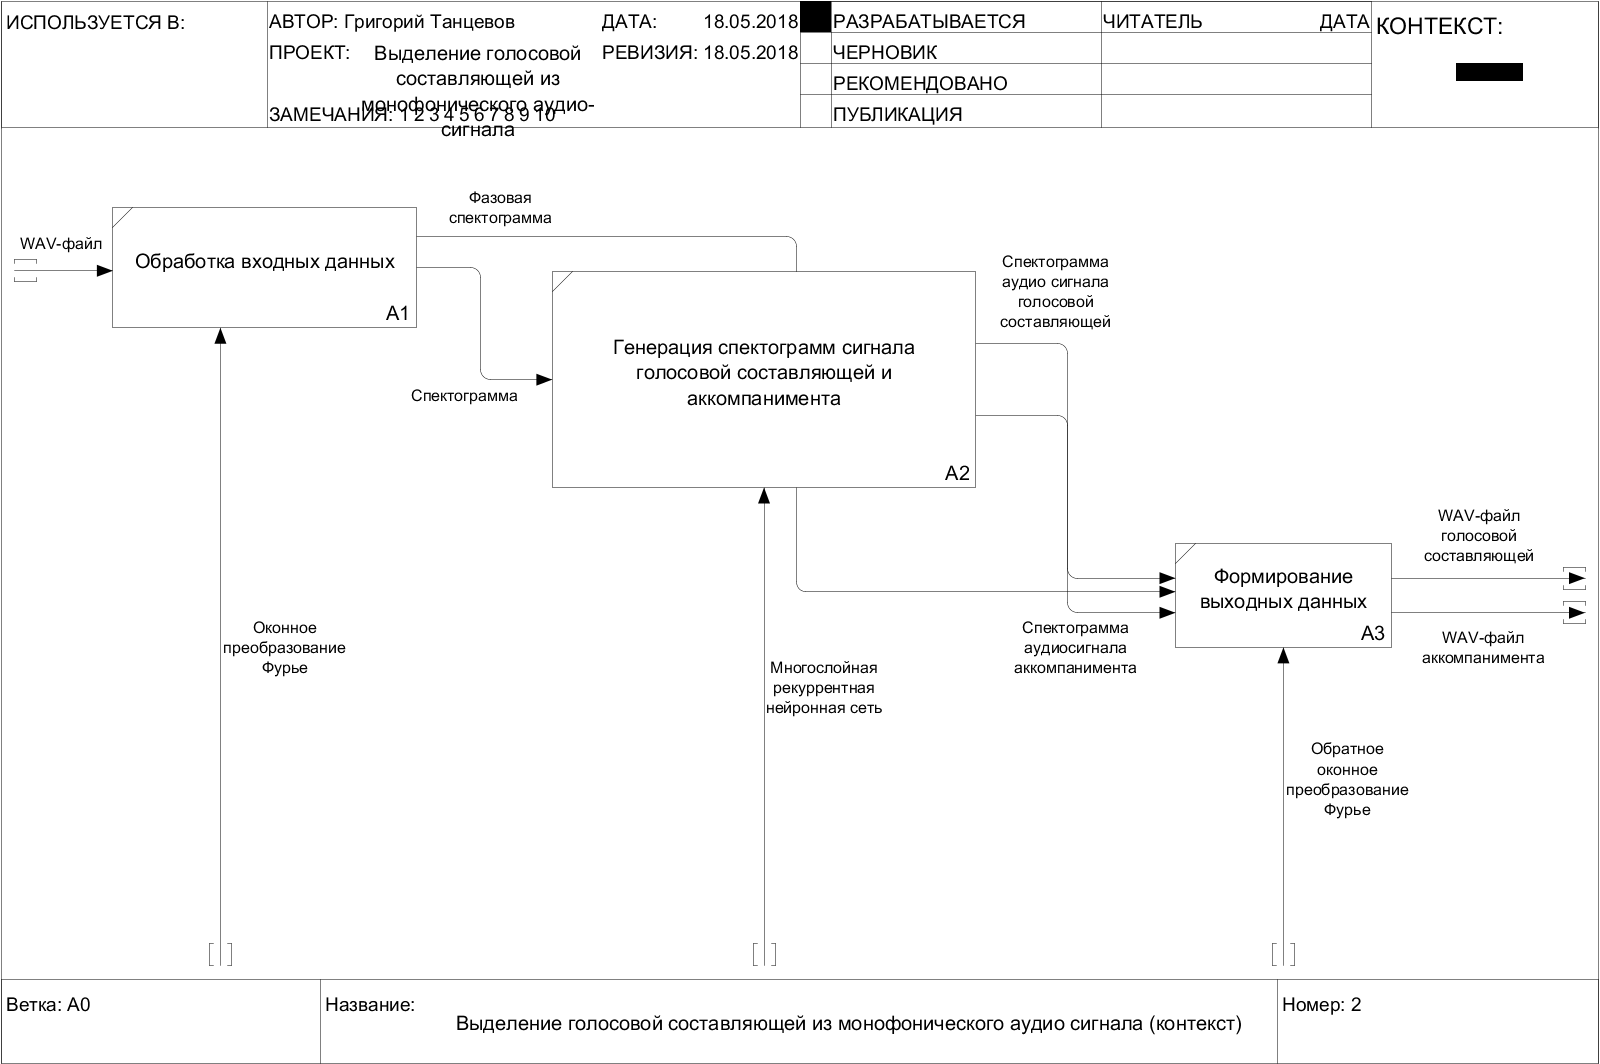
\includegraphics[width=\textwidth]{inc/img/02_A0}
	\caption{IDEF0 программного продукта}
	\label{des:idef0}
\end{figure}

\section{Алгоритмы}

\subsection{Обработка входных данных}

Чтение аудио-файлов, хранящиеся в формате WAVE, происходит с помощью библиотеки. Результатом работы библиотечной функции является информация о частоте дискретизации и структура со значениями амплитуд сигнала. 

После считывания аудио-файла происходит построение его спектра при помощи оконного преобразования Фурье. Результатом работы этого алгоритма является структура, в которой хранятся наборы частот по отрезкам времени.

В качестве оконной функции используется Окно Ханна, дискретная функция которого которого записывается следующим образом:

\begin{equation}
w(n) = 0.5 - 0.5 \cos \Big(\frac{2\pi n}{N-1}\Big)
\end{equation}

\subsection{Генерация частотно-временных масок}

Для получения частотно-временных масок используется многослойная рекурентная нейронная сеть. На ее вход подается результат применения ОПФ к исходному сигналу. Результатом работы сети являются спектограммы выделяемых источников.

\subsection{Описание сети}

\begin{figure}
	\centering
	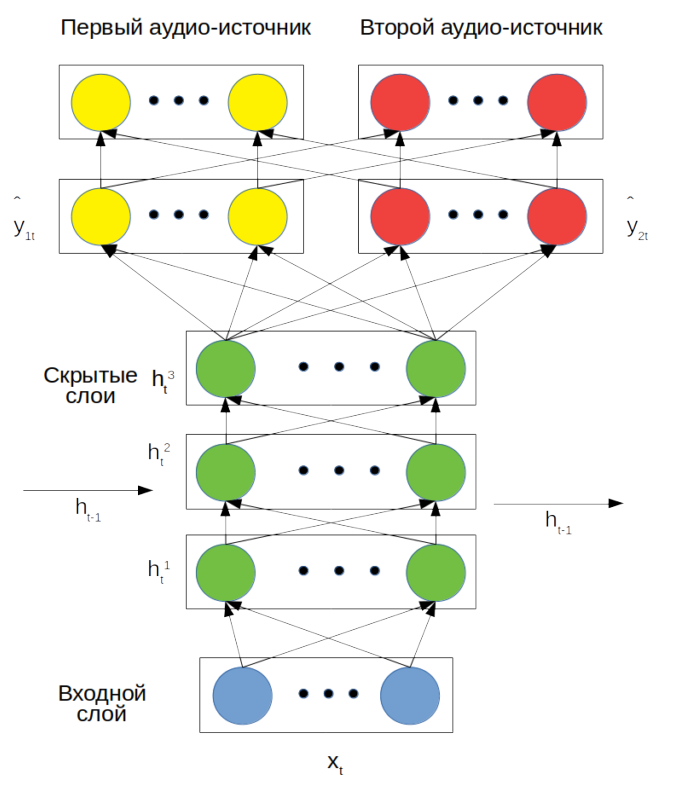
\includegraphics[width=0.5\textwidth]{inc/img/drnn-design}
	\caption{Схема нейронной сети}
	\label{des:drnn}
\end{figure}

Многослойная РНС состоит из 6 слоев:

\begin{enumerate}
	\item Входной слой. На вход подается спектограмма исходного сигнала, полученная в следствии применения ОПФ.
	\item 3 скрытых слоя $h_t^1, h_t^2$ и $h_t^3$. 
	
	Слой $h_t^2$ имеет рекурентную связь. Отсюда результатом работы этого слоя в момент времени $t$ можно записать как:
	
	\begin{equation}
	h_t^2 = f_h(x_t, h_{t-1}^2) = \sigma_2 (U^2 h_{t-1}^2 + W^2(h_{t}^1))
	\end{equation}
	
	где:
	
	\begin{itemize}
		\item $W^i$ -- веса связей, идущих от предшествующего слоя;
		\item $U^i$ -- веса рекуррентой связи;
		\item $h_t^{i-1}$ -- результат работы предшествующего слоя;
		\item $\sigma_i$ -- активационная функция.
	\end{itemize}

	Так как у первого слоя предшествующий слой -- входной, то его результать вычисляется по следующей формуле:
	
	\begin{equation}
	h_t^1 = \sigma_1 ( W^1 x_t)
	\end{equation}
	
	Результатом работы слоя $h_t^3$ будет:
	
	\begin{equation}
	h_t^3 = \sigma_3 (W^2 h_t^2)
	\end{equation}
	
	В качестве активационной функции используется ReLU (формула \ref{anal:relu}).
	
	\item Слой генерации частотно-временных масок. Данный слой использует результат работы слоя третьего рекуррентного слоя для генерации двух векторов $\hat{y}_{1t}$ и $\hat{y}_{2t}$, размер которых равен размеру входного вектора. Данные последовательности используются для вычисления частотно-временной маски $m_t(f)$, которая является функцией частоты:
	
	\begin{equation}
	m_t(f) = \frac{|\hat{y}_{1t}(f)|}{|\hat{y}_{1t}(f)| + |\hat{y}_{1t}(f)|}
	\label{des:mask}
	\end{equation}
	
	\item Слой генерации спектограмм. Для получение спектограм выделяемых источников к спектограмме исходного аудио-сигнала применяется частотно-временная маска, полученная на предыдущем слое. В итоге получаются два вектора $\tilde{y}_{1t}$ и $\tilde{y}_{2t}$, вычисляющиемя как:
	
	\begin{equation}
	\tilde{y}_{1t}(f) = m(f)x_t(f)
	\end{equation}
	
	
	\begin{equation}
	\tilde{y}_{2t}(f) = (1 - m(f))x_t(f)
	\end{equation}
	
	С учетом формулы \ref{des:mask}:
	
	\begin{equation}
	\tilde{y}_{1t} = \frac{|\hat{y}_{1t}|}{|\hat{y}_{1t}| + |\hat{y}_{1t}|} \bigodot x_t
	\end{equation}
	
	
	\begin{equation}
	\tilde{y}_{2t} = \frac{|\hat{y}_{2t}|}{|\hat{y}_{1t}| + |\hat{y}_{1t}|} \bigodot x_t
	\end{equation}
	
\end{enumerate}

Схема нейронной сети представлена на рисунке \ref{des:drnn}.

\subsubsection{Обучение нейронной сети}

Для обучения нейронной сети используется Метод обратного распространения ошибки. Для вычисления ошибок между сгенерированными векторами $ \tilde{y}_{1t}, \tilde{y}_{2t} $ и ожидаемыми $ y_{1t}, y_{2t} $ используются среднеквадратичное отклонение

\begin{equation}
J_{MSE} = || \tilde{y}_{1t} - y_{1t} ||^2 + || \tilde{y}_{2t} - y_{2t} ||^2
\end{equation}

и дивергенция Кулбека-Лейблера

\begin{equation}
J_{KL} = D(y_{1t}, \tilde{y}_{1t}) + D(y_{2t}, \tilde{y}_{2t})
\end{equation}

где $D$ вычисляется по формуле \ref{anal:kl}.

\subsection{Формирование выходных данных}

Для формирования WAV-файлов используется обратное оконное преобразование Фурье. В качестве параметров передается матрица, полученная из спектограммы выделяемого источника и фазовой спектограммы исходного сигнала.

\section{Используемые структуры данных}

Для хранения данных WAV-файла используется последовательность действительных чисел, хранящая информацию об уровне сигнала в определенным момент времени.

Для хранения результатов ОПФ и работы нейронной сети используется матрица комплексных чисел, так как требуется быстрый доступ к элементам, а изменений размеров после первичного заполнения не происходит. 

Комплексное число представляет собой структуру с двумя полями: реальной и мнимой частями.

В качестве входных данных нейронной сети используется используется амплитудная характеристика спектограммы, харнящаяся в виде матрицы действительных чисел фиксированного размера.

\section{Тестирование}

Тестирование программного продукта заключается в сравнении результата работы методов на тестовых наборах данных с заранее заданным результатом. Тестовые наборы данных (англ. dataset) для проверки работы алгоритмов, связанных с обработкой музыкальных произведений, предоставляются в открытом доступе в Интернете.

Важной характеристикой входных данных является стиль вокала, так как разные стили имеют разные спектральные характеристики. Можно выделить следующие классы эквивалентности:

\begin{itemize}
	\item академический вокал(классический, оперный);
	\item эстрадный вокал;
	\item джазовый вокал;
	\item рок вокал;
	\item народное пение;
	\item горловое пение.
\end{itemize}

Следует протестировать работу алгоритмов на музыкальных произведениях с эстрадным вокалом.

\subsection{Тестовые данные}

Для тестированя программного продукта используется открытый набор данных DSD100 (Community-Based Signal Separation Evaluation Campaign 2016). В DSD100 содержатся 100 музыкальных произведений разных жанров, с мужским и женским вокалом. Каждый музыкальный трек был сведен с использованием профессиональных средств звукозаписи.

DSD100 состоит из WAV-файлов сведенных музыкальных произведений, хранящихся в папке <<Mixture>>, и WAV-файлов источников, хранящихся в папке <<Sources>>.

Источники разделены на 4 типа:

\begin{itemize}
	\item вокал;
	\item бас;
	\item ударные;
	\item остальное.
\end{itemize}

Все записи являются полифоническими (двух-канальными).

Для тестирования разработанного метода данный датасет необходимо привести к следующему виду. Все источники приводятся в монофонический формат. Бас, ударные и остальное объединяются в один WAV-файл.

%%% Local Variables:
%%% mode: latex
%%% TeX-master: "rpz"
%%% End:
